\documentclass[a4paper]{article}
%\usepackage[ngerman]{babel}
\usepackage[T1]{fontenc}
\usepackage[utf8]{inputenc}
\usepackage{textcomp}
\usepackage{geometry}
\geometry{ left=2cm, right=2cm, top=2cm, bottom=3cm, bindingoffset=5mm}
\usepackage{graphicx}
\usepackage{xcolor}
\usepackage{hyperref}
\usepackage{longtable}
\usepackage{amstext}
\usepackage{array}
\usepackage{amsmath}
\newcolumntype{L}{>{$}l<{$}}
\usepackage{tabularx, ragged2e}
\usepackage{helvet}
\renewcommand{\familydefault}{\sfdefault}
\usepackage{lastpage}
\usepackage{todonotes}
\usepackage{titlesec}
\titleformat*{\section}{\large\bfseries}
\usepackage{listings}
\usepackage{color}

\usepackage{tikz}
%\newcommand{\tikzmark}[2]{\tikz[overlay, remember picture] \node[inner sep=0pt, outer sep=0pt, anchor=base] (#1) {#2};}
\usetikzlibrary{tikzmark}


\definecolor{mygreen}{rgb}{0.18, 0.545, 0.341}
\definecolor{mygray}{rgb}{0.5,0.5,0.5}
\definecolor{myblue}{rgb}{0.53,0.61,0.85}

\lstset{
 keywordstyle=\color{mygreen},
 commentstyle=\color{mygray},
 numbers=left,
 numbersep=5pt, 
 numberstyle=\scriptsize\color{mygray}
 }

\usepackage{amsmath,amssymb}

\DeclareRobustCommand{\bbone}{\text{\usefont{U}{bbold}{m}{n}1}}

\DeclareMathOperator{\EX}{\mathbb{E}}% expected value

\date{}
\author{}
\usepackage{fancyhdr}
\pagestyle{fancy}
\fancyhf{}
\fancyhead[R]{Felix Burk\\ Pascal Huszár}
\fancyhead[L]{Reinforcment Learning \\ Summer Term 2021 }
\fancyfoot[R]{page \thepage \text{ }/ \pageref*{LastPage}}
%\fancyfoot[LE]{Seite \thepage \text{ }von \pageref{LastPage}}
\renewcommand{\headrulewidth}{0.5pt}

\usepackage{amsmath}
\DeclareMathOperator*{\argmax}{arg\,max}
\DeclareMathOperator*{\argmin}{arg\,min}


\title{\textbf{Exercise 07}}

\begin{document}
	\maketitle 
	\thispagestyle{fancy}
	
    \section*{Task 1 - Planning and Learning}
    	\subsection*{a)}    
    		As for n-step Sarsa (seen below) an action value is strengthen (during the episode) based on the future actions until the state at position n.	
\begin{figure}[!ht]
	\centering
	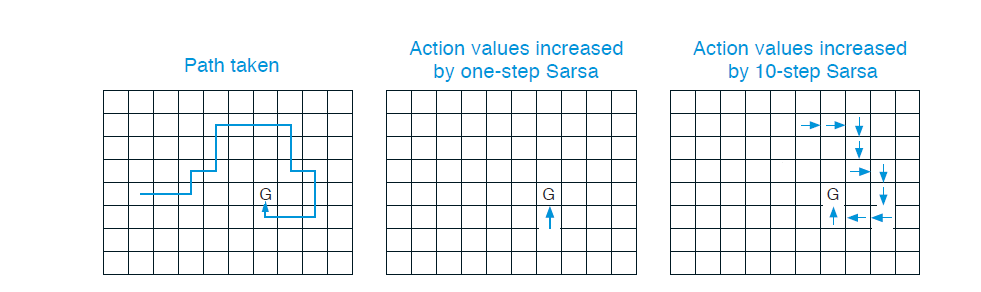
\includegraphics[width=0.8\linewidth]{n-step_sarsa} 
	\caption{Gridworld example for n-step sarsa. Figure from the book RL by Sutton and Barto (Fig. 7.4)}
	\label{fig:n-step_sarsa}
\end{figure}
\\
In the case of Dyna-Q the Q(s, a) is update with the learned model n-times. Furthermore through sampling previously observed states (planning), in just a small number of episodes an extensive policy can be developed (seen below). While the n-step sarsa only strengthen visited states, dyna-q updates Q(s, a) by applying the model.
\begin{figure}[!h]
	\centering
	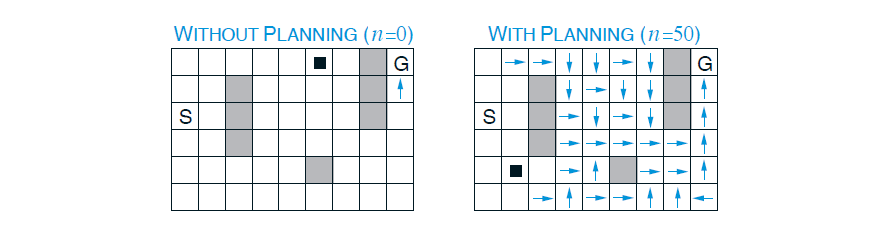
\includegraphics[width=0.8\linewidth]{dyna-q} 
	\caption{Gridworld example for dyna-q. Figure from the book RL by Sutton and Barto (Fig. 8.3)}
	\label{fig:n-step_sarsa}
\end{figure}
\newpage 
The tree backup algorithms considers more information during an episode. Instead of just updating the value of a node by the discounted rewards alogn the path with "end" node the idea is to also add the action values for each intermediate node (along the path).
But it also does not sample like the dyn-q approach and also it would a memory expensive task to store all the aciton values under a large n
\begin{figure}[!h]
	\centering
	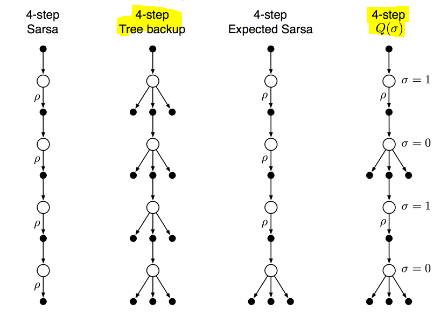
\includegraphics[width=0.6\linewidth]{tree-backup_Q-omega} 
	\caption{Gridworld example for dyna-q. Figure from the book RL by Sutton and Barto (Fig. 8.3)}
	\label{fig:n-step_sarsa}
\end{figure}
    	\subsection*{b)} 
\end{document}